% !TeX spellcheck = de_CH_frami

\section{Wavelets\label{sec:sgwt:wavelets}}
\rhead{Wavelets}

Standard-Basis: Lokalisiert Ort

EF-Basis: delokalisiert Frequenz


\begin{figure}
    \centering
    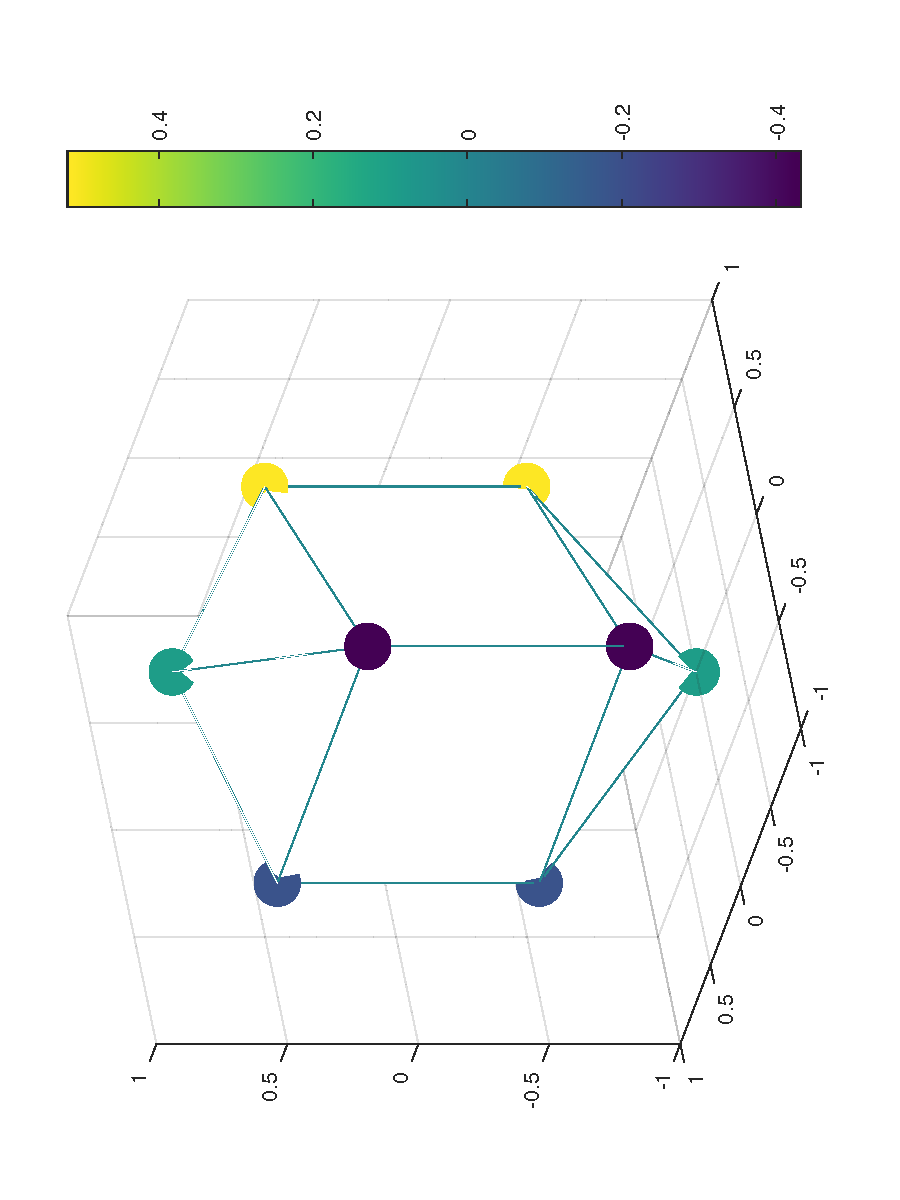
\includegraphics[
    angle=-90,
    origin=c,
    scale=0.7
    ]{papers/sgwt/images/graph-chi-4.pdf}
    \vspace{-80pt}
    \caption{Dreidimensionale Darstellung des Kugelgraphen. Die Funktionswerte 
        werden dabei mit Farben auf den Knoten dargestellt. 
        \label{fig:sgwt:sphere:graph:chi}}
\end{figure}

\begin{figure}
    \centering
    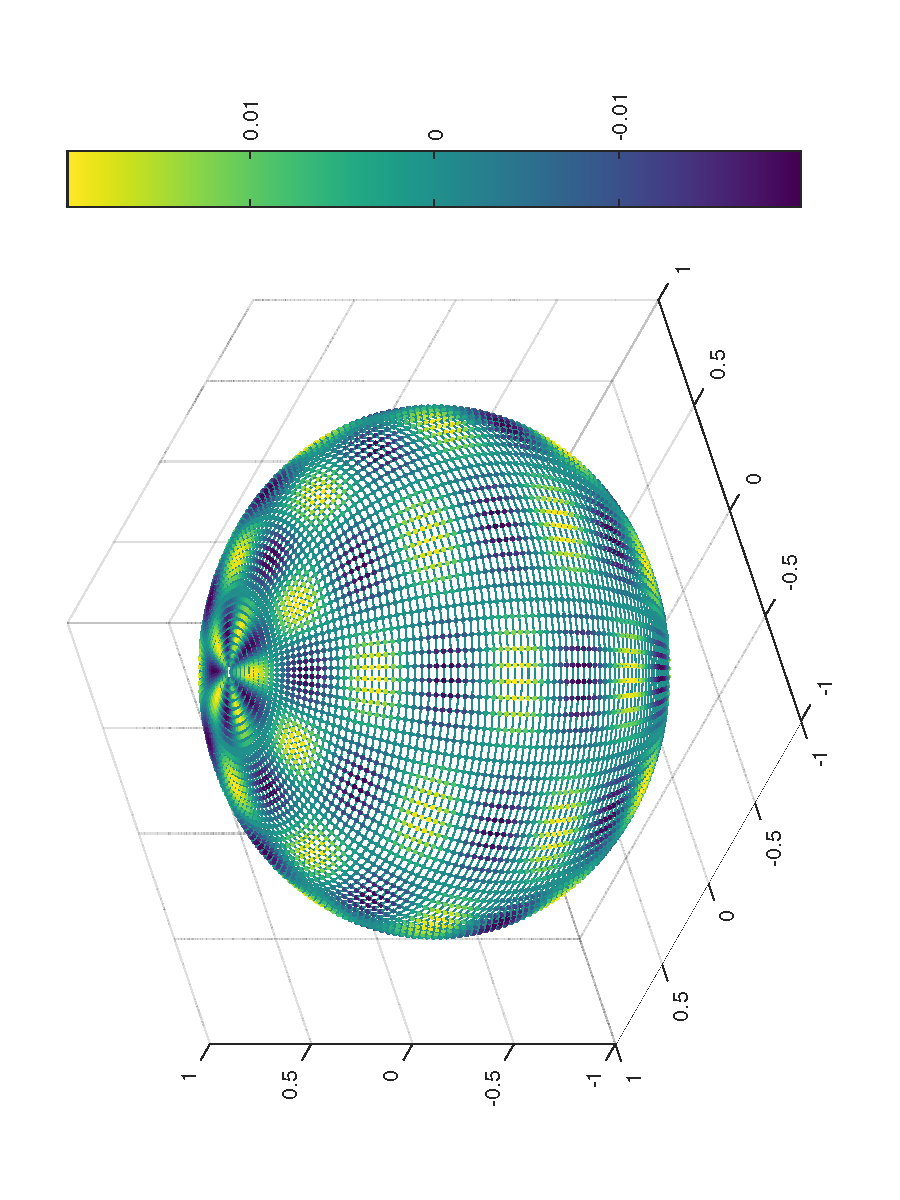
\includegraphics[
    angle=-90,
    origin=c,
    scale=0.7
    ]{papers/sgwt/images/graph-100-100-chi-150.pdf}
    \vspace{-80pt}
    \caption{Kugelgraph mit $l = b = 100$. Darstellung von $\chi_{150}$.
        \label{fig:sgwt:sphere:graph:chi:hh}}
\end{figure}

